\documentclass{article}
\usepackage{url,graphicx}

\newcommand{\BEASTVersion}{2.0}
\newcommand{\TracerVersion}{1.5}
\newcommand{\FigTreeVersion}{1.3.1}

\bibliographystyle{cell}


\begin{document}
\title{Ancestral Reconstruction/Discrete Phylogeography with BEAST 2.0}
\author{Remco Bouckaert \url{remco@cs.auckland.ac.nz}}
\maketitle

\section{Introduction}


In this tutorial we describe a full Bayesian framework for phylogeography developed in  \cite{Lemey:2009uq}.

You will need the following software at your disposal:

\begin{itemize}

\item {\bf BEAST} - this package contains the BEAST program, BEAUti, TreeAnnotator and other utility programs. This tutorial is written for BEAST v{\BEASTVersion}, which has support for multiple partitions. It is available for download from \\* \texttt{http://beast2.cs.auckland.ac.nz/}.
\item {\bf Tracer} - this program is used to explore the output of BEAST (and other Bayesian MCMC programs). It graphically and
quantitively summarizes the distributions of continuous parameters and provides diagnostic information. At the time of
writing, the current version is v{\TracerVersion}. It is available for download from \texttt{http://beast.bio.ed.ac.uk/}.
\item {\bf FigTree} - this is an application for displaying and printing molecular phylogenies, in particular those obtained using
BEAST. At the time of writing, the current version is v{\FigTreeVersion}. It is available for download from \texttt{http://tree.bio.ed.ac.uk/}.
\item {\bf Spread} for summarysing the geographic spread in a KML file (available from \url{http://www.kuleuven.ac.be/aidslab/phylogeography/SPREAD.html}.
\item {\bf google-earth} for displaying the KML file (just google for it, if you have not already have it installed).
\end{itemize}


This tutorial guides you through a discrete phylogegraphy analysis of a H5N1 epidemic in South China.
The data is a subset of a larger set compiled by \cite{wallace:2007st}.
It consists of 43 sequences of 1698 characters.

We go through the following steps:
\begin{itemize}
\item The first step is to install the beast-classic add-on that contains the phylogegraphic models. 
\item Then, we use BEAUti to set up the analysis, and write it to an XML file.
\item We use BEAST to run the MCMC analysis based on the XML file.
\item The results will need to be checked for convergence using Tracer.
\item Finally, we post-process the output of the MCMC so we can visualise the geographical dispersion.
\end{itemize}

\subsubsection*{Set up BEAUti for phylogeography}

Phylogeography as described in this tutorial is part of the {\tt beast-classic} add-on.
To install the add-on, run BEAUti by double clicking on its icon. 
Select the File/Manage Add-ons menu. A dialog pops up showing the add-ons already installed. 

\begin{center}
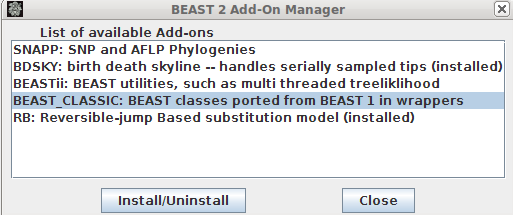
\includegraphics[scale=0.4]{figures/addonmgr.png}
\end{center}


Select the BEAST-CLASSIC entry in the list, and click the Install button. After a little while the dialog is updated and it shows that the add-on is now installed.
BEAST-CLASSIC requires BEASTii, so if you have not already installed BEASTii, an error message may be shown warning that BEASTii should be installed as well.

\begin{center}
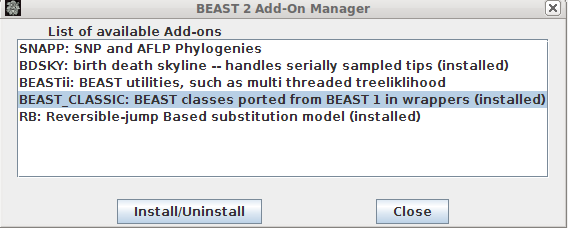
\includegraphics[scale=0.4]{figures/addonmgr2.png}
\end{center}



\subsection*{BEAUti}


\subsubsection*{Loading the NEXUS file }

To load a NEXUS format alignment, simply select the \texttt{Import
Alignment} option from the File menu: 

Select the file called \texttt{H5N1.nex}. The file contains an alignment of sequences. The \texttt{H5N1.nex} looks like this (content has been truncated):

\begin{verbatim}
#NEXUS
BEGIN DATA;
       DIMENSIONS  NTAX =47 NCHAR=2811;
       FORMAT DATATYPE = DNA GAP = - MISSING = ?;
       MATRIX 	
hOH10_97.2_41.053_80.706  TTCCCTATCTACACAATACCAGACAAGCTA...
hWVa01_93.2_40.505_80.575 TTCCCTATCTACACAATACCAGACAAGCTA...
NY01_03.4_41.057_73.794   TTCCCTATCTACACAATACCAGACAAGCTA...
NY03_03.4_42.934_76.565   TTCCCTATCTACACAATACCAGACAAGCTA...
NY04_03.4_42.617_75.037   TTCCCTATCTACACAATACCAGACAAGCTA...
NY12_03.4_42.996_78.170   TTCCCTATCTACACAATACCAGACAAGCTA...
         ... ...

;
END;
\end{verbatim}

\medskip{}

Once loaded, a partition is displayed in the main panel.
You can double click any alignment (partition) to show its detail.

\begin{figure}
\begin{center}

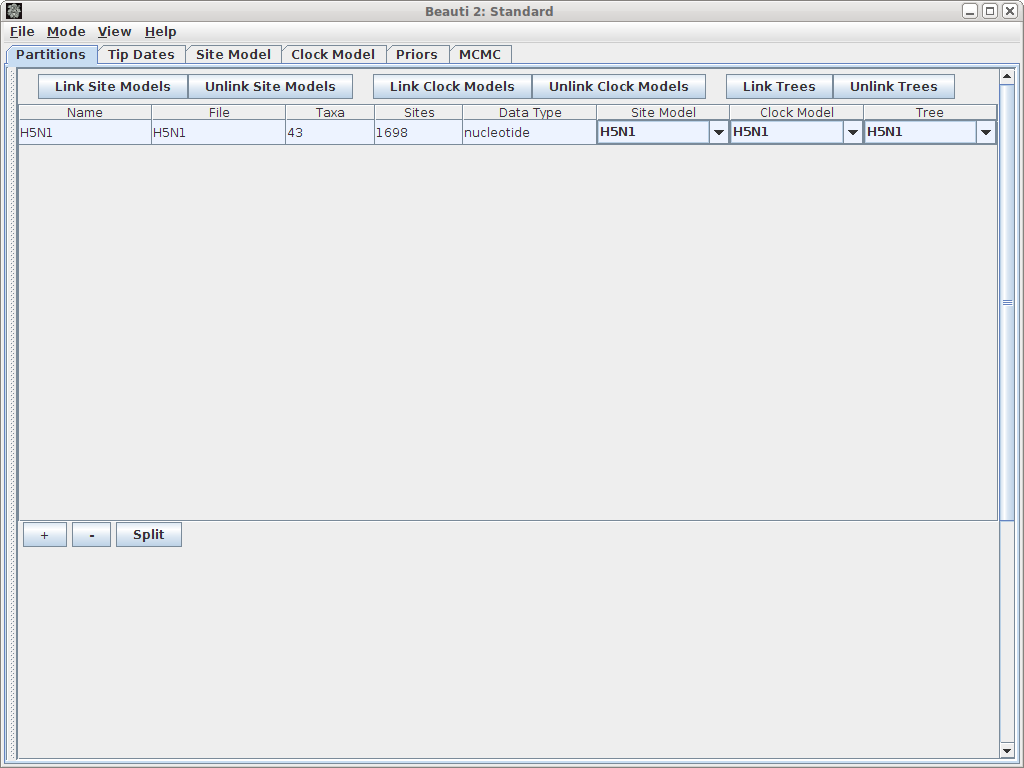
\includegraphics[scale=0.4]{figures/BEAUti_DataPartitions}

\end{center}
\caption{\label{fig.datapartition} Data partition panel after loading alignment.}
\end{figure}

\subsubsection*{Set up dates}

We want to use tip dates for this analysis.

Select the 'Tip Dates' tab, and click the 'Use tip dates' check box.

Since we can derive the date from the taxon names, click the 'Guess' button.

A dialog pops up, where we can specify the dates as follows: the dates are encoded after the last underscore in the name.
So, we want to use everything after the last underscore, as shown in Figure \ref{fig.dates}.

\begin{figure}
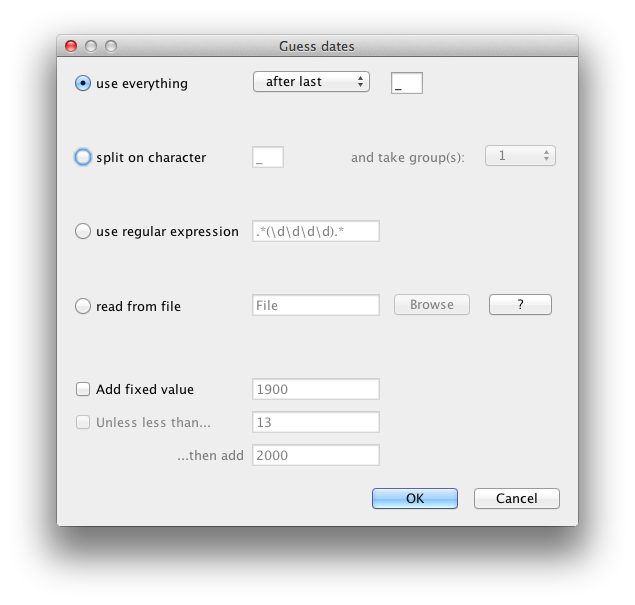
\includegraphics[scale=0.4]{figures/BEAUti_dates.png}
\caption{\label{fig.dates}Setting up the dates for H5N1}
\end{figure}

Click OK and the dates are populated by the correct value. Always double check that this happened correctly and no strange outliers or wrong encodings cause any problems, of course.

\subsubsection*{Setting the substitution model}

Select the Site model tab, and change the site model to HKY, and frequency model to `empirical'.

Also, set the gamma category count to 4, and check the estimate box on the 'Shape' parameter that now pops up.
The screen should look like this:

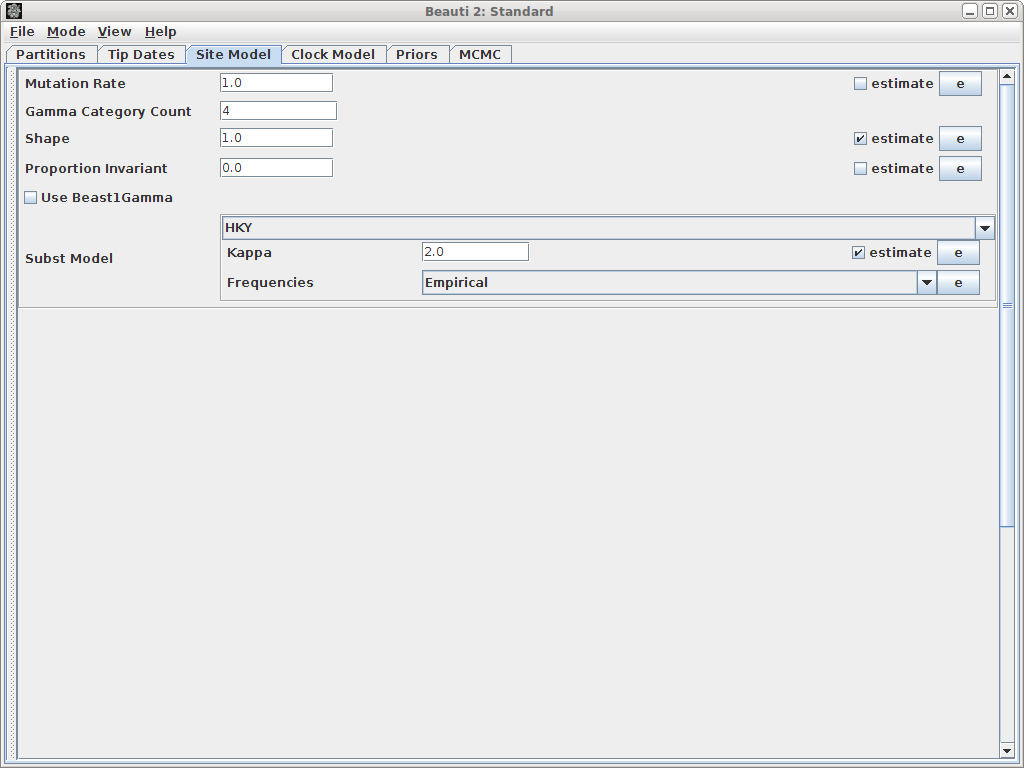
\includegraphics[scale=0.4,clip=true,trim=0 300 0 0]{figures/BEAUti_sitemodel.png}

\subsubsection*{Setting the clock model}

We use a strict clock, but to make the analysis converge a bit quicker, we fix the clock rate to 0.004.
First, click the menu Mode, and unset 'Automatically set clock rate'. Then, uncheck the estimate flag on the clock rate, and change the rate to 0.004.
The screen should look like this:

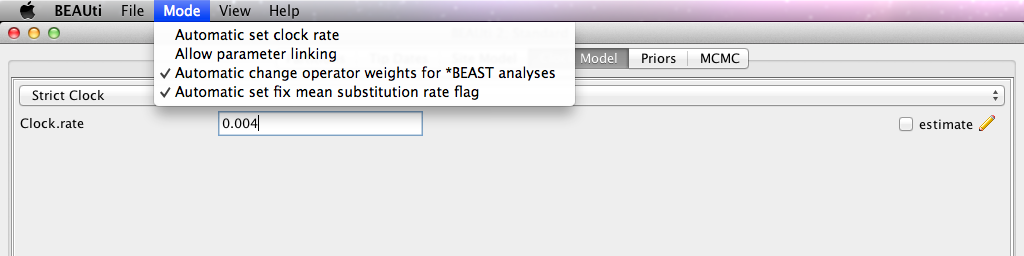
\includegraphics[scale=0.4,clip=true,trim=0 300 0 0]{figures/BEAUti_clockmodel.png}


\subsubsection*{Priors}

Change the tree prior from Yule to Coalescent with Constant Population. The other priors are fine. The screen should look like this:

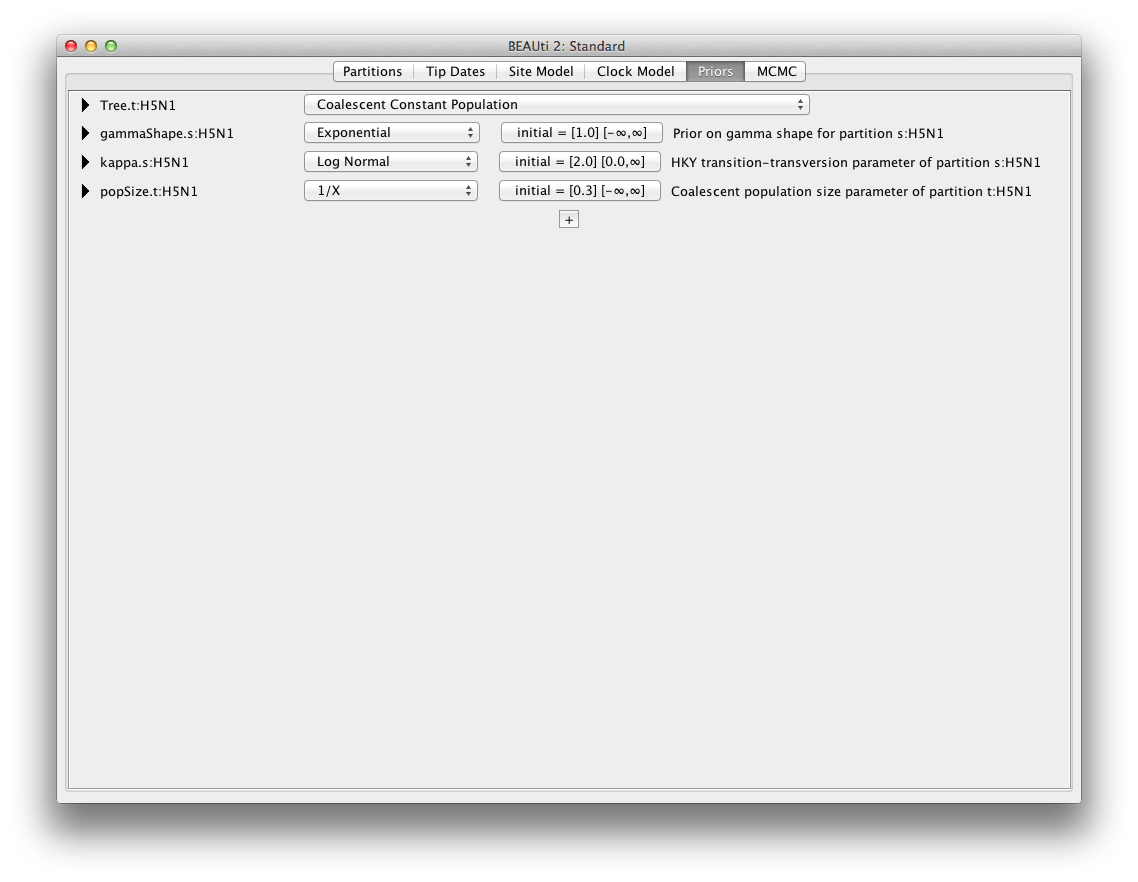
\includegraphics[scale=0.4,clip=true,trim=0 300 0 0]{figures/BEAUti_priors.png}


\subsubsection*{Setting up a discrete trait}

Go to the Partitions tab, and click the + button at the bottom of the screen.
If the installation of the beast-classic add-on went OK, a dialog pops up, where you can select what to add.

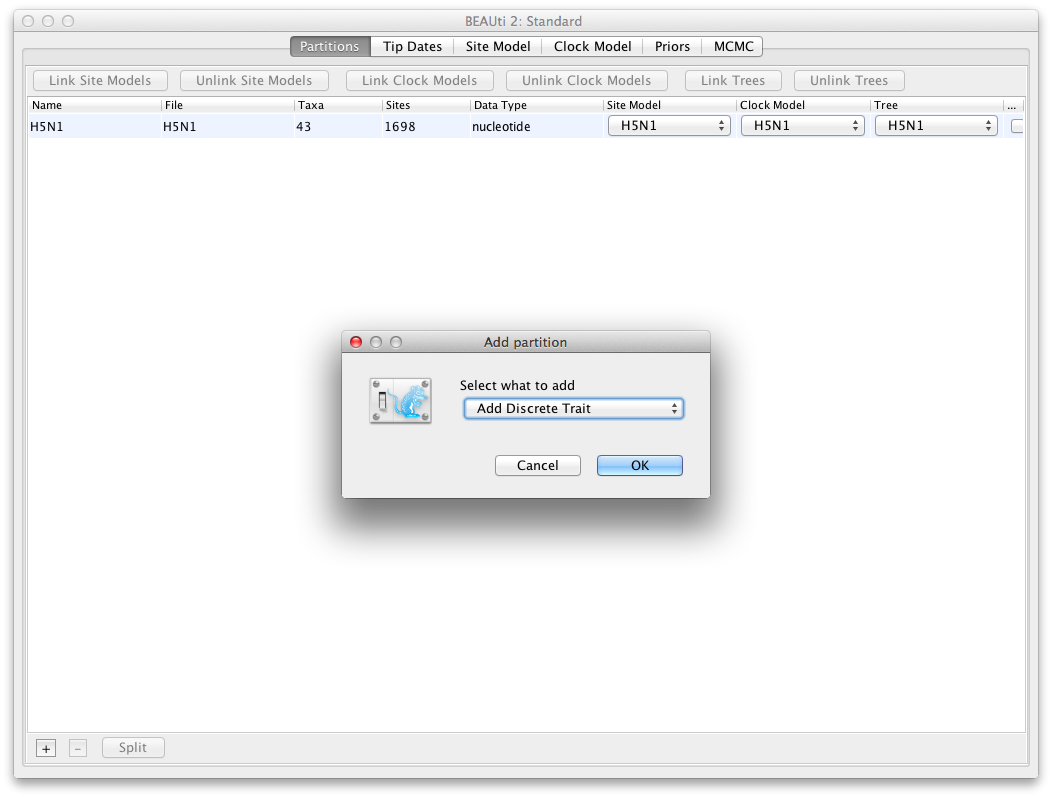
\includegraphics[scale=0.4]{figures/BEAUti_trait.png}

Select 'discrete trait' and click OK. Now you can give a name to the trait, and select a tree to associate the trait with. 
Here we will use 'location'.

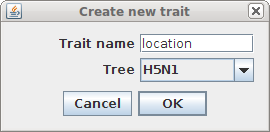
\includegraphics[scale=0.4,clip=true,trim=240 200 240 200]{figures/BEAUti_trait2.png}

Change the name and click OK. Now, a dialog pops up where you can manually add the locations. However, the location is already encoded in the name, so we can `guess' it. Click the Guess button and a dialog pops up where we can choose to define the names by splitting on underscore and select the third group. Before you click OK, the screen should look like this:

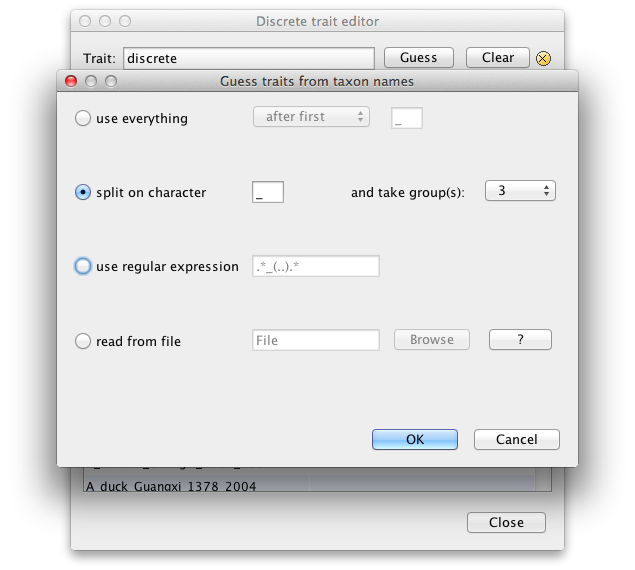
\includegraphics[scale=0.4,clip=true,trim=260 60 260 60]{figures/BEAUti_trait3.png}

After clicking OK, the list is populated by locations, like so:

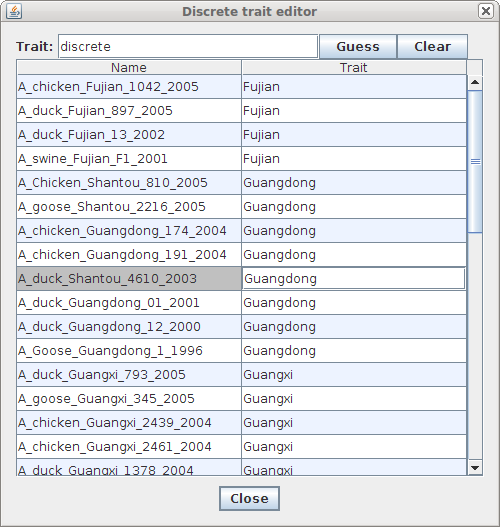
\includegraphics[scale=0.4,clip=true,trim=260 60 260 60]{figures/BEAUti_trait4.png}

You want to double check that all locations are indeed the ones you want, because it is easy for an irregularity to creep into taxon names, and the guess-work may not be correct.
Click close, and the data partitions panel has a new partition added for location.

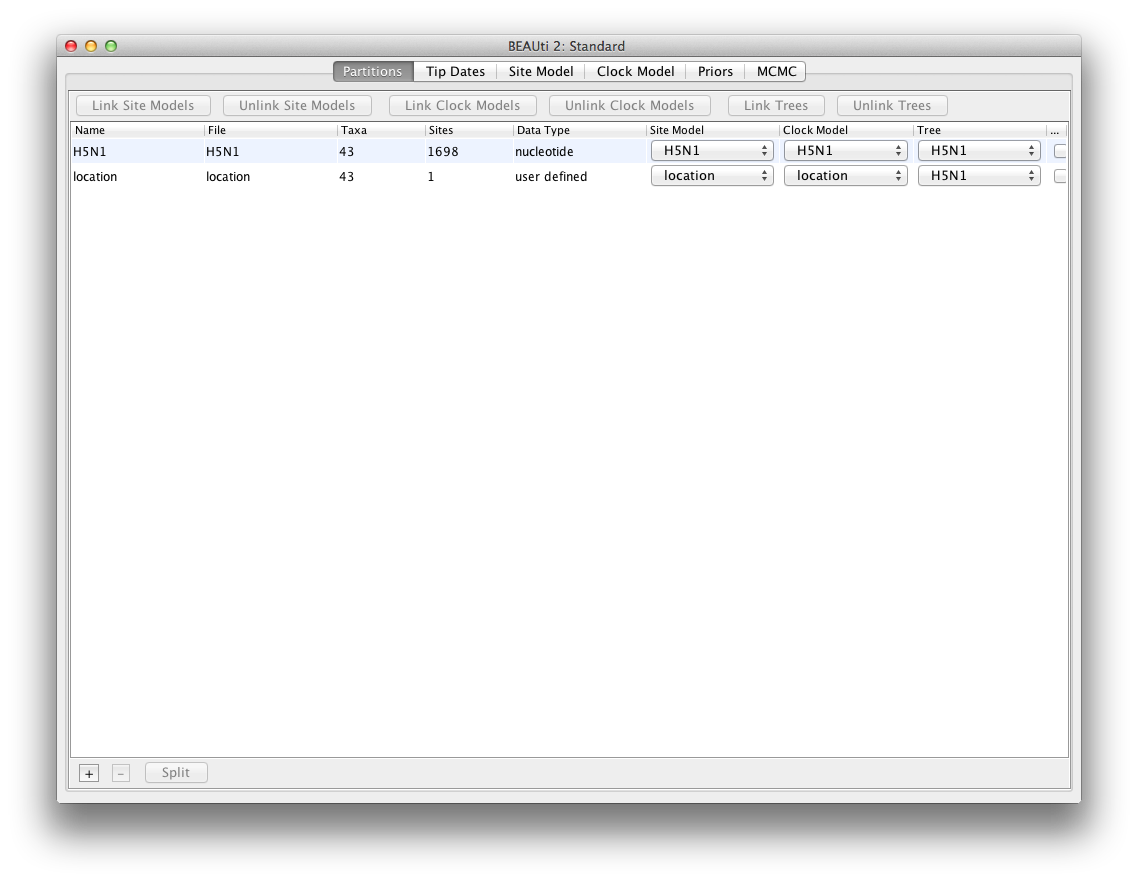
\includegraphics[scale=0.4]{figures/BEAUti_DataPartitions2.png}

To get the trait edit dialog back, double click the location partition.

\subsubsection*{Setting the clock model}

Click the clock model tab, and select the 'location' on the left.
This shows the strict clock for the trait.

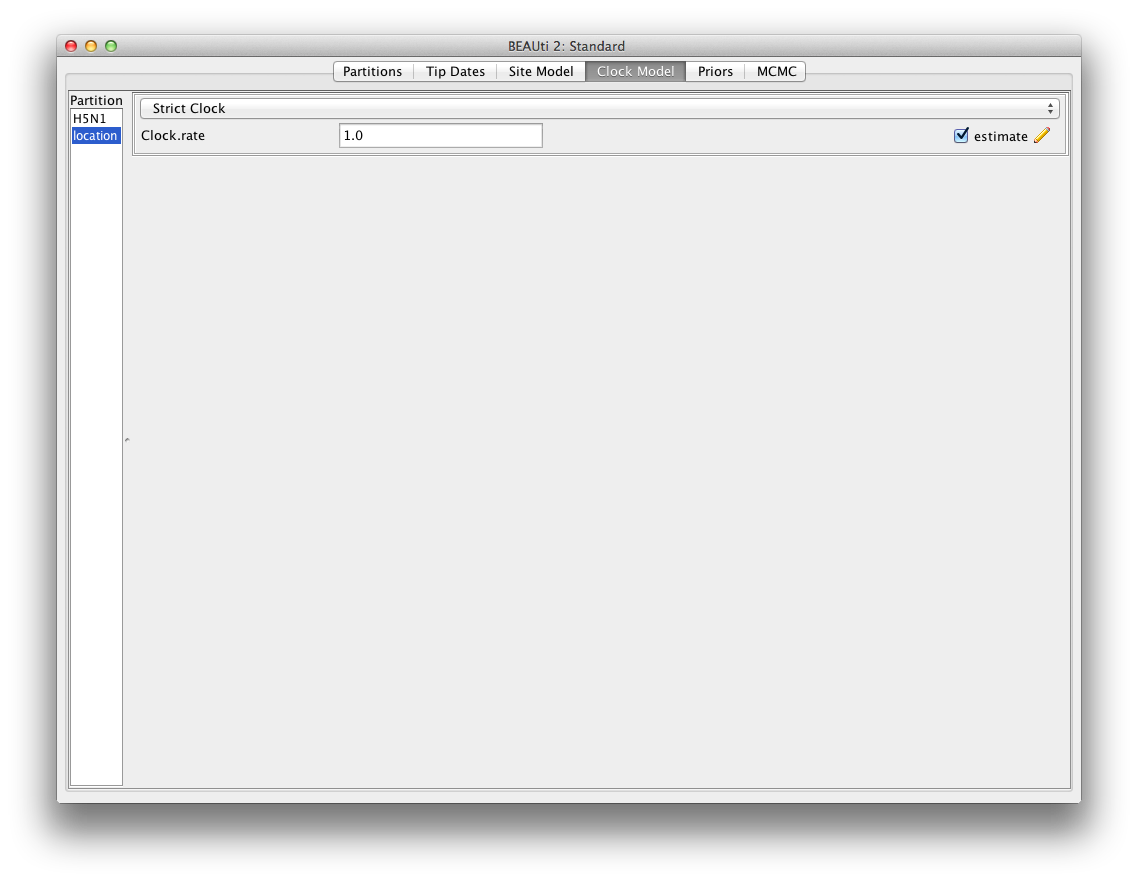
\includegraphics[scale=0.4,clip=true,trim=0 300 0 0]{figures/BEAUti_clockmodel2.png}

\subsubsection*{Priors}

Click the priors tab, to show the extra priors added for the discrete analysis.

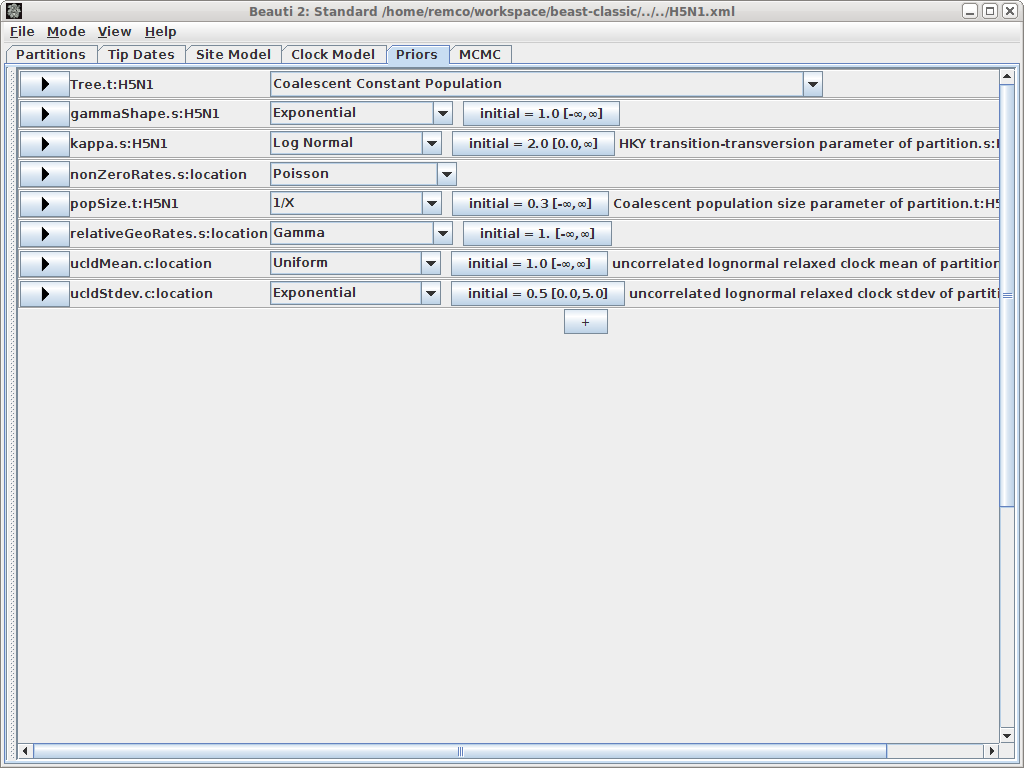
\includegraphics[scale=0.4,clip=true,trim=0 200 0 0]{figures/BEAUti_priors2.png}

\subsubsection*{Setting the MCMC options }

The next tab, {\bf MCMC}, provides more general
settings to control the length of the MCMC and the file names. 

Firstly we have the \textbf{Length of chain}. This is the number of
steps the MCMC will make in the chain before finishing. The appropriate length of the chain depends on the size of the data set, the complexity of the
model and the accuracy of the answer required. The default value of 10,000,000
is entirely arbitrary and should be adjusted according to the size
of your data set. For this data set let's initially set the chain
length to 3,000,000 as this will run reasonably quickly on most modern
computers (less than 10 minutes).

The next options specify how often the parameter values in the Markov
chain should be displayed on the screen and recorded in the log file.
The screen output is simply for monitoring the programs progress so
can be set to any value (although if set too small, the sheer quantity
of information being displayed on the screen will actually slow the
program down). For the log file, the value should be set relative
to the total length of the chain. Sampling too often will result in
very large files with little extra benefit in terms of the precision
of the analysis. Sample too infrequently and the log file will not
contain much information about the distributions of the parameters. 
You probably want to aim to store no more than 10,000 samples so this should be
set to no less than chain length / 10,000.

For this exercise we will set the screen log to 100000 and the file log to 2000. The final two
options give the file names of the log files for the sampled parameters and
the trees. These will be set to a default based on the name of the
imported NEXUS file. 

\begin{figure}
\begin{center}

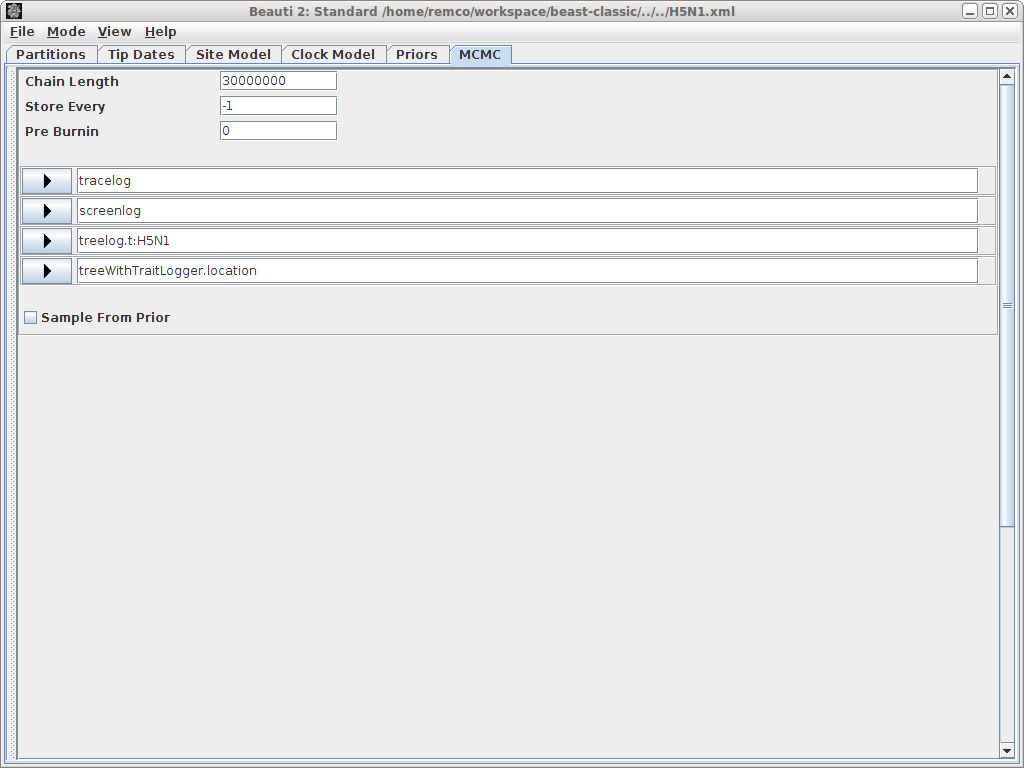
\includegraphics[scale=0.4,clip=true,trim=0 200 0 0]{figures/BEAUti_MCMC}

\end{center}
\caption{\label{fig.MCMC} Setting up the MCMC paremeters.}
\end{figure}


If you are using windows then we suggest you add the suffix \texttt{.txt} to both of these (so,
\texttt{gopher.log.txt} and \texttt{gopher.trees.txt}) so that Windows recognizes
these as text files. 











\subsubsection*{Generating the BEAST XML file }

We are now ready to create the BEAST XML file. To do this, either select the {\bf File/Save} or {\bf File/Save As} option from the \textbf{File} menu. Check the default priors setting and click \textbf{Continue}. Save the file with an appropriate name (we usually end the filename with \texttt{.xml}, i.e., \texttt{RacRABC.xml}). We are now ready to run the file through BEAST. 

\subsection*{Running BEAST }

Now run BEAST and when it asks for an input file, provide your newly
created XML file as input by click \textbf{Choose File ...}, and then click \textbf{Run}. 

\begin{figure}
\begin{center}

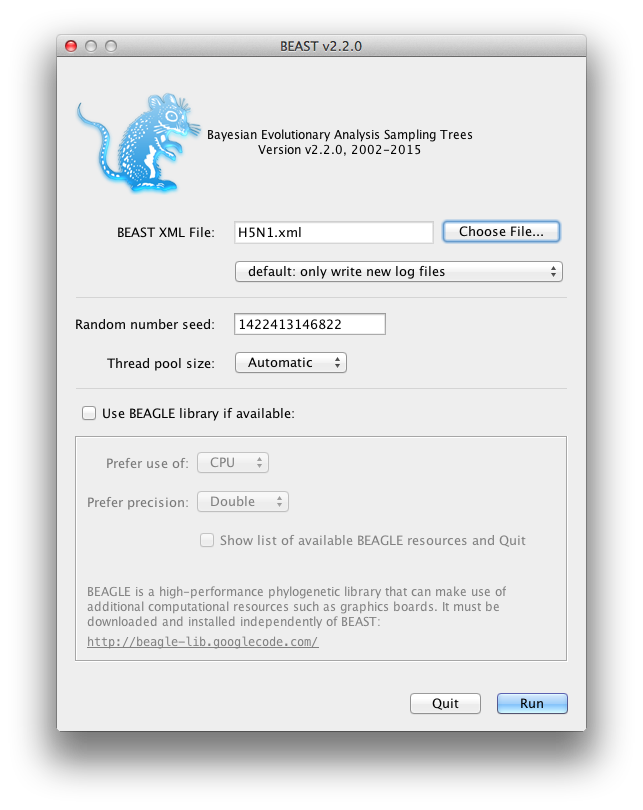
\includegraphics[scale=0.5]{figures/BEAST}

\end{center}
\caption{\label{fig.BEAST} Launching BEAST.}
\end{figure}


BEAST will then run until it has finished
reporting information to the screen. The actual results files are
saved to the disk in the same location as your input file. The output to the screen will
look something like this: 

{\scriptsize   
\begin{verbatim}

          BEAST v2.0.e Prerelease r794, 2002-2011
       Bayesian Evolutionary Analysis Sampling Trees
                 Designed and developed by
Remco Bouckaert, Alexei J. Drummond, Andrew Rambaut and Marc A. Suchard
                              
               Department of Computer Science
                   University of Auckland
                  remco@cs.auckland.ac.nz
                  alexei@cs.auckland.ac.nz
                              
             Institute of Evolutionary Biology
                  University of Edinburgh
                     a.rambaut@ed.ac.uk
                              
              David Geffen School of Medicine
           University of California, Los Angeles
                     msuchard@ucla.edu
                              
                Downloads, Help & Resources:
              	http://beast2.cs.auckland.ac.nz
                              
Source code distributed under the GNU Lesser General Public License:
              	http://code.google.com/p/beast2
                              
                     BEAST developers:
	Alex Alekseyenko, Trevor Bedford, Erik Bloomquist, Joseph Heled, 
	Sebastian Hoehna, Denise Kuehnert, Philippe Lemey, Wai Lok Sibon Li, 
	Gerton Lunter, Sidney Markowitz, Vladimir Minin, Michael Defoin Platel, 
          	Oliver Pybus, Chieh-Hsi Wu, Walter Xie
                              
                         Thanks to:
    	Roald Forsberg, Beth Shapiro and Korbinian Strimmer

File: H5N1.xml seed: 1347411445277 threads: 1

Random number seed: 1347411445277

... ...

\end{verbatim}}

\subsection*{Analysing the results}

Run the program called {\bf Tracer} to analyze the output of BEAST. When the main
window has opened, choose {\bf Import Trace File...} from the {\bf File} menu and select the file that
BEAST has created called \texttt{H5N1.123123.log} where 123123 is the seed you used.
You should now see a window like in Figure \ref{fig.tracer}.

\begin{figure}
\begin{center}

\frame{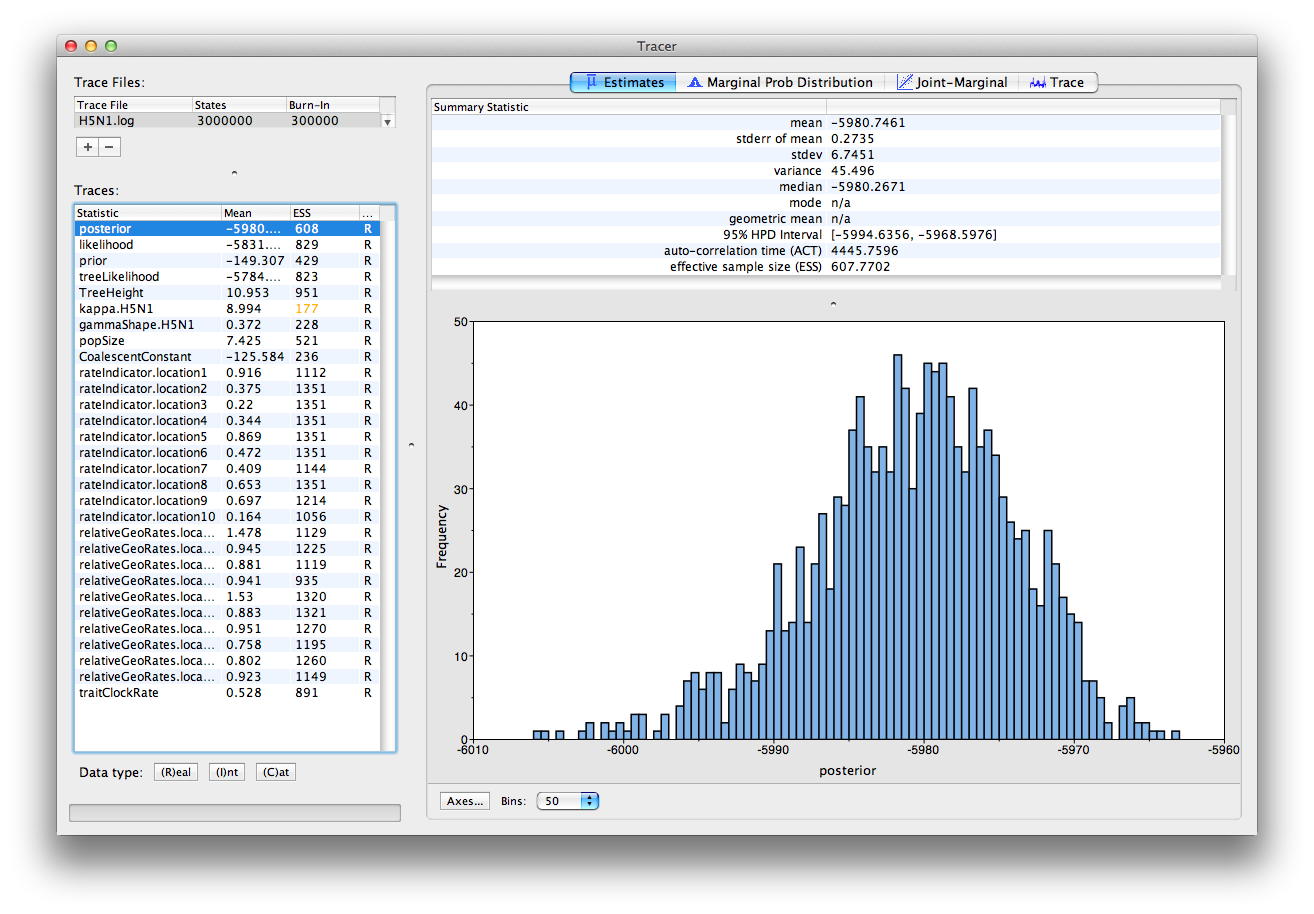
\includegraphics[scale=0.4]{figures/Tracer}}

\end{center}
\caption{\label{fig.tracer} Tracer with the H5N1 data.}
\end{figure}


Remember that MCMC is a stochastic algorithm so the actual numbers will not be exactly the same.

On the left hand side is a list of the different quantities that BEAST has logged. There are traces for the posterior (this
is the log of the product of the tree likelihood and the prior probabilities), and the continuous parameters. Selecting a trace
on the left brings up analyses for this trace on the right hand side depending on tab that is selected. When first opened, the
`posterior' trace is selected and various statistics of this trace are shown under the Estimates tab.
In the top right of the window is a table of calculated statistics for the selected trace. 

Tracer will plot a (marginal posterior) distribution for the selected parameter and also give you statistics such as the mean and median. The \texttt{95\% HPD lower} or \texttt {upper} stands for {\it highest posterior density interval} and represents the most compact interval on the selected parameter that contains 95\% of the posterior probability. It can be thought of as a Bayesian analog to a confidence interval. 

\subsection*{Obtaining an estimate of the phylogenetic tree}

BEAST also produces a sample of plausible trees. 
These can be summarized using the program {\bf TreeAnnotator}. This will take the set of trees and identify a single tree that best represents the posterior distribution. It will then annotate this selected tree topology with the mean ages of all the
nodes as well as the 95\% HPD interval of divergence times for each clade in the selected tree. It will also calculate the posterior clade probability for each
node. Run the {\bf TreeAnnotator} program and set it up to look like in Figure \ref{fig.TreeAnnotator}.

\begin{figure}
\begin{center}

\frame{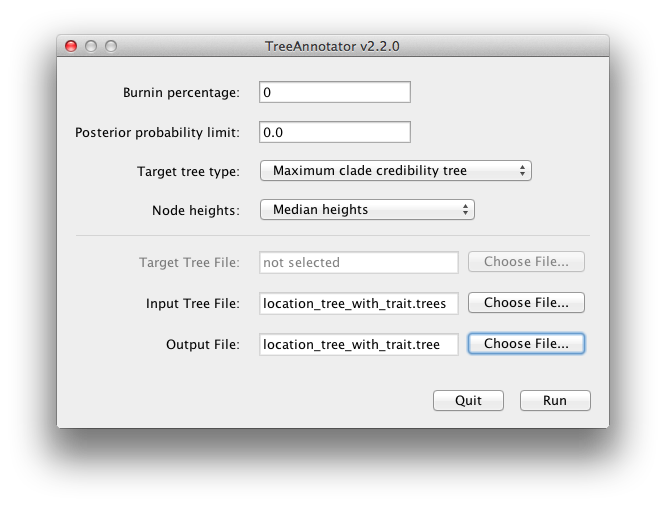
\includegraphics[scale=0.4]{figures/TreeAnnotator}}

\end{center}
\caption{\label{fig.TreeAnnotator} Using TreeAnnotator to summarise the tree set.}
\end{figure}


The burnin is the number of trees to remove from the start of the sample. Unlike {\bf Tracer} which specifies the number of steps as a burnin, in {\bf TreeAnnotator} you need to specify the actual number of trees. For this run, we use the default setting.

The {\bf Posterior probability limit} option specifies a limit such that if a node is found at less than this frequency in the sample of trees (i.e., has a posterior probability less than this limit), it will not be annotated. The default of 0.5 means that only nodes seen in the majority of trees will be annotated. Set this to zero to annotate all nodes.

For {\bf Target tree type} you can either choose a specific tree from a file or ask TreeAnnotator to find a tree in your sample. The default option, {\bf Maximum clade credibility tree}, finds the tree with the highest product of the posterior probability of all its nodes.

Choose {\bf Mean heights} for node heights. This sets the heights (ages) of each node in the tree to the mean height across the entire sample of trees for that clade.

For the input file, select the trees file that BEAST created (by default this will be called \texttt{gopher.species.trees}) and select a file for the output (here we called it \texttt{gopher.species.tree}).

Now press \texttt{Run} and wait for the program to finish.

\subsection*{Distribution of root location}

When you open the summary tree in a text editor, and look at the end of the tree definition, grab the last entry for location.set and location.set.prob. They might look something like this:
\\
{\tt
location.set = \{"Hunan","Guangxi","Fujian","HongKong","Guangdong"\}
location.set.prob = \{0.024983344437041973, 0.16822118587608262, 0.05463024650233178, 0.6085942704863424, 0.1435709526982012\}
}

This means that we have the following distribution for the root location:

\begin{tabular}{l|l}
\hline
location & probability\\
\hline
Hunan&0.024983344437041973\\
Guangxi&0.16822118587608262\\
Fujian&0.05463024650233178\\
HongKong&0.6085942704863424\\
Guangdong&0.1435709526982012\\
\hline
\end{tabular}

This distribution shows that the 95\% HPD consists of all locations except Hunan, with a 
strong indication that Hong-Kong might be the root with over 60\% probability. It is quite
typical that a lot of locations are part of the 95\% HPD in discrete phylogeography.

\subsection*{Viewing the Sprecies Tree}

We can look at the tree in another program called {\bf FigTree}. Run this program, and open
the \texttt{summary.tree} file by using the Open command in the File menu. The tree should appear.
You can now try selecting some of the options in the control panel on the left. Try selecting
{\bf Appearance} to get colour on the branches by location. Also, you can set the branch width
according to posterior support. You should end up with something like Figure \ref{fig.figtree}.

\begin{figure}
\begin{center}

\frame{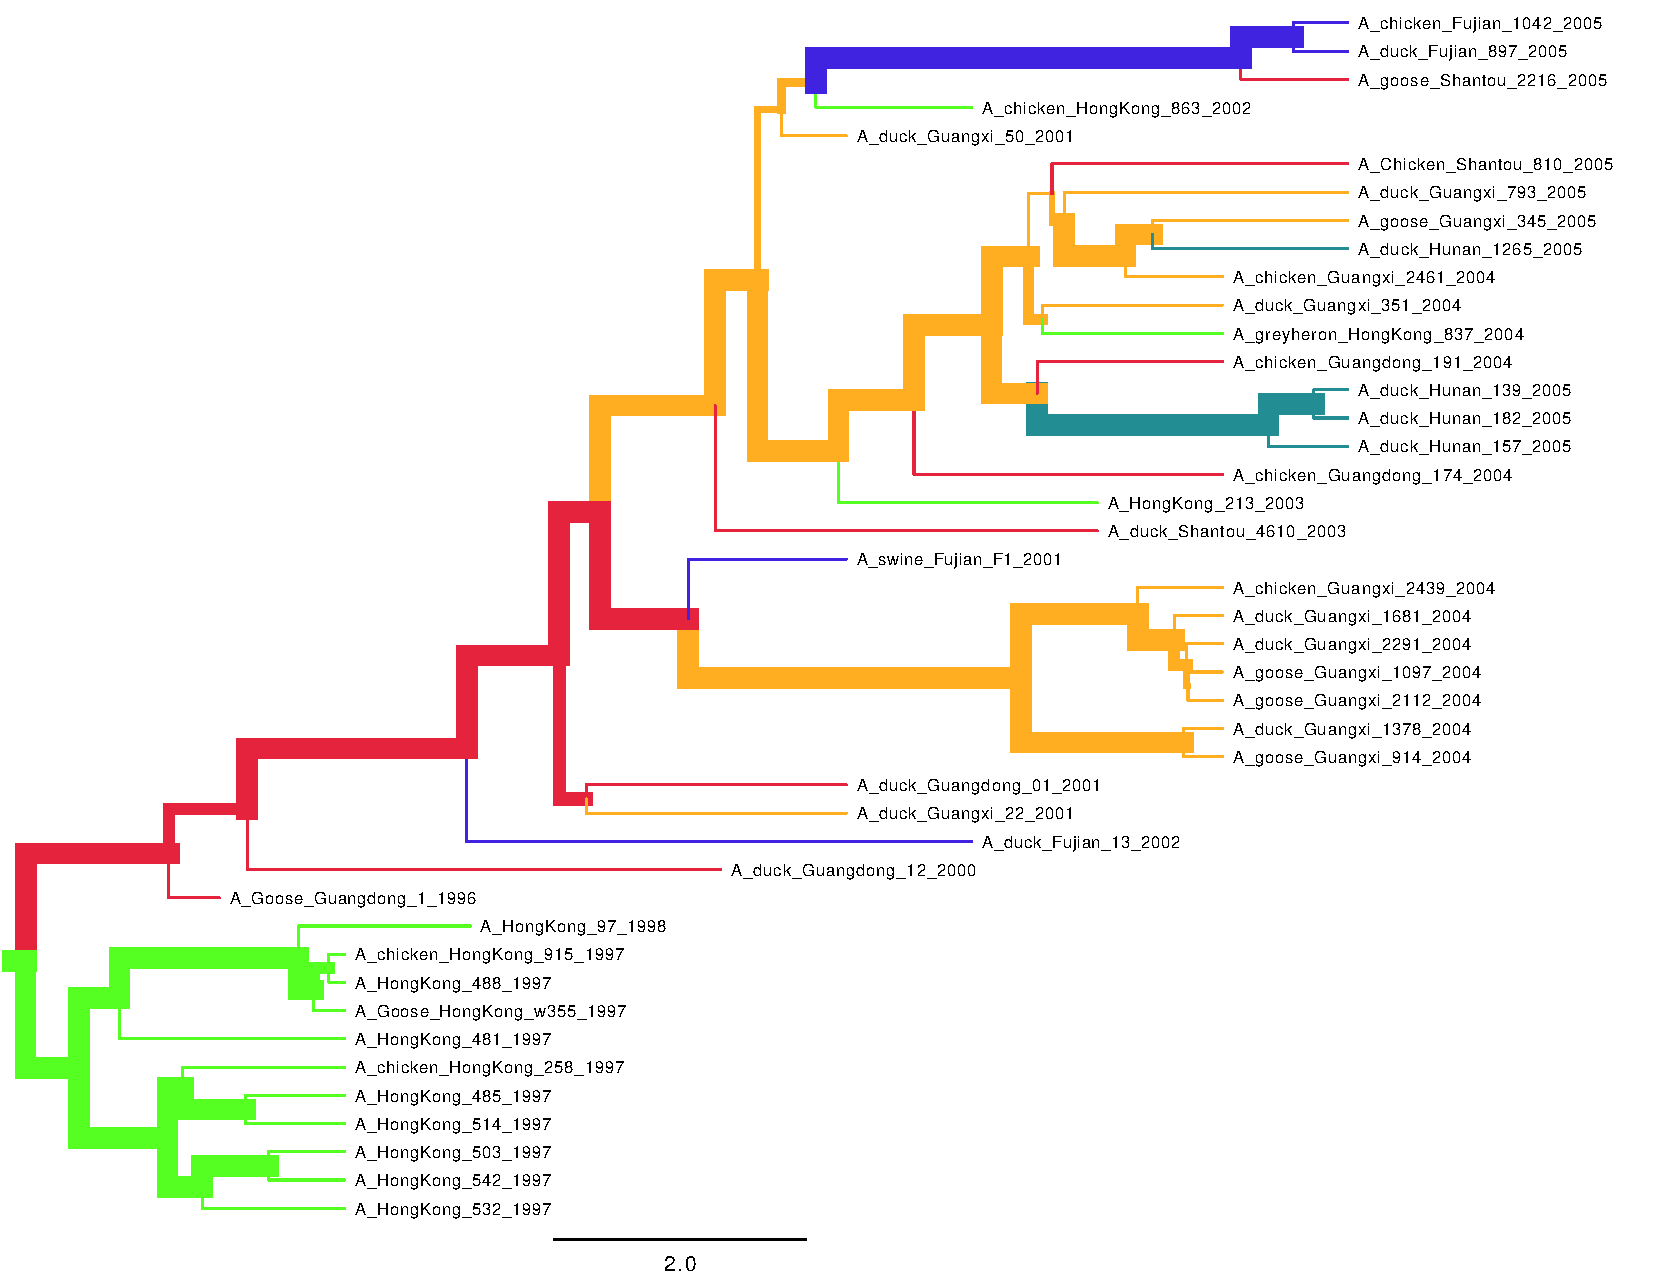
\includegraphics[scale=0.4]{figures/figtree.pdf}}

\end{center}
\caption{\label{fig.figtree} Figtree representation of the summary tree. Branch colours represent location
and branch widths posterior support for the branch.}
\end{figure}


Alternatively, you can load the species tree set (note this is NOT the summary tree, but the complete set) into DensiTree and set it up as follows.

\begin{itemize}
\item Set burn-in to 300. The tree should not be collapsed any more.
\item Show a root-canal tree to guide the eye. 
\item Show a grid, and play with the grid options to only show lines at 2 year intervals covering round numbers (that is, 2000, instead of 2001.22).
\end{itemize}

The image should look something like Figure \ref{fig.DensiTree}.

\begin{figure}
\begin{center}
\frame{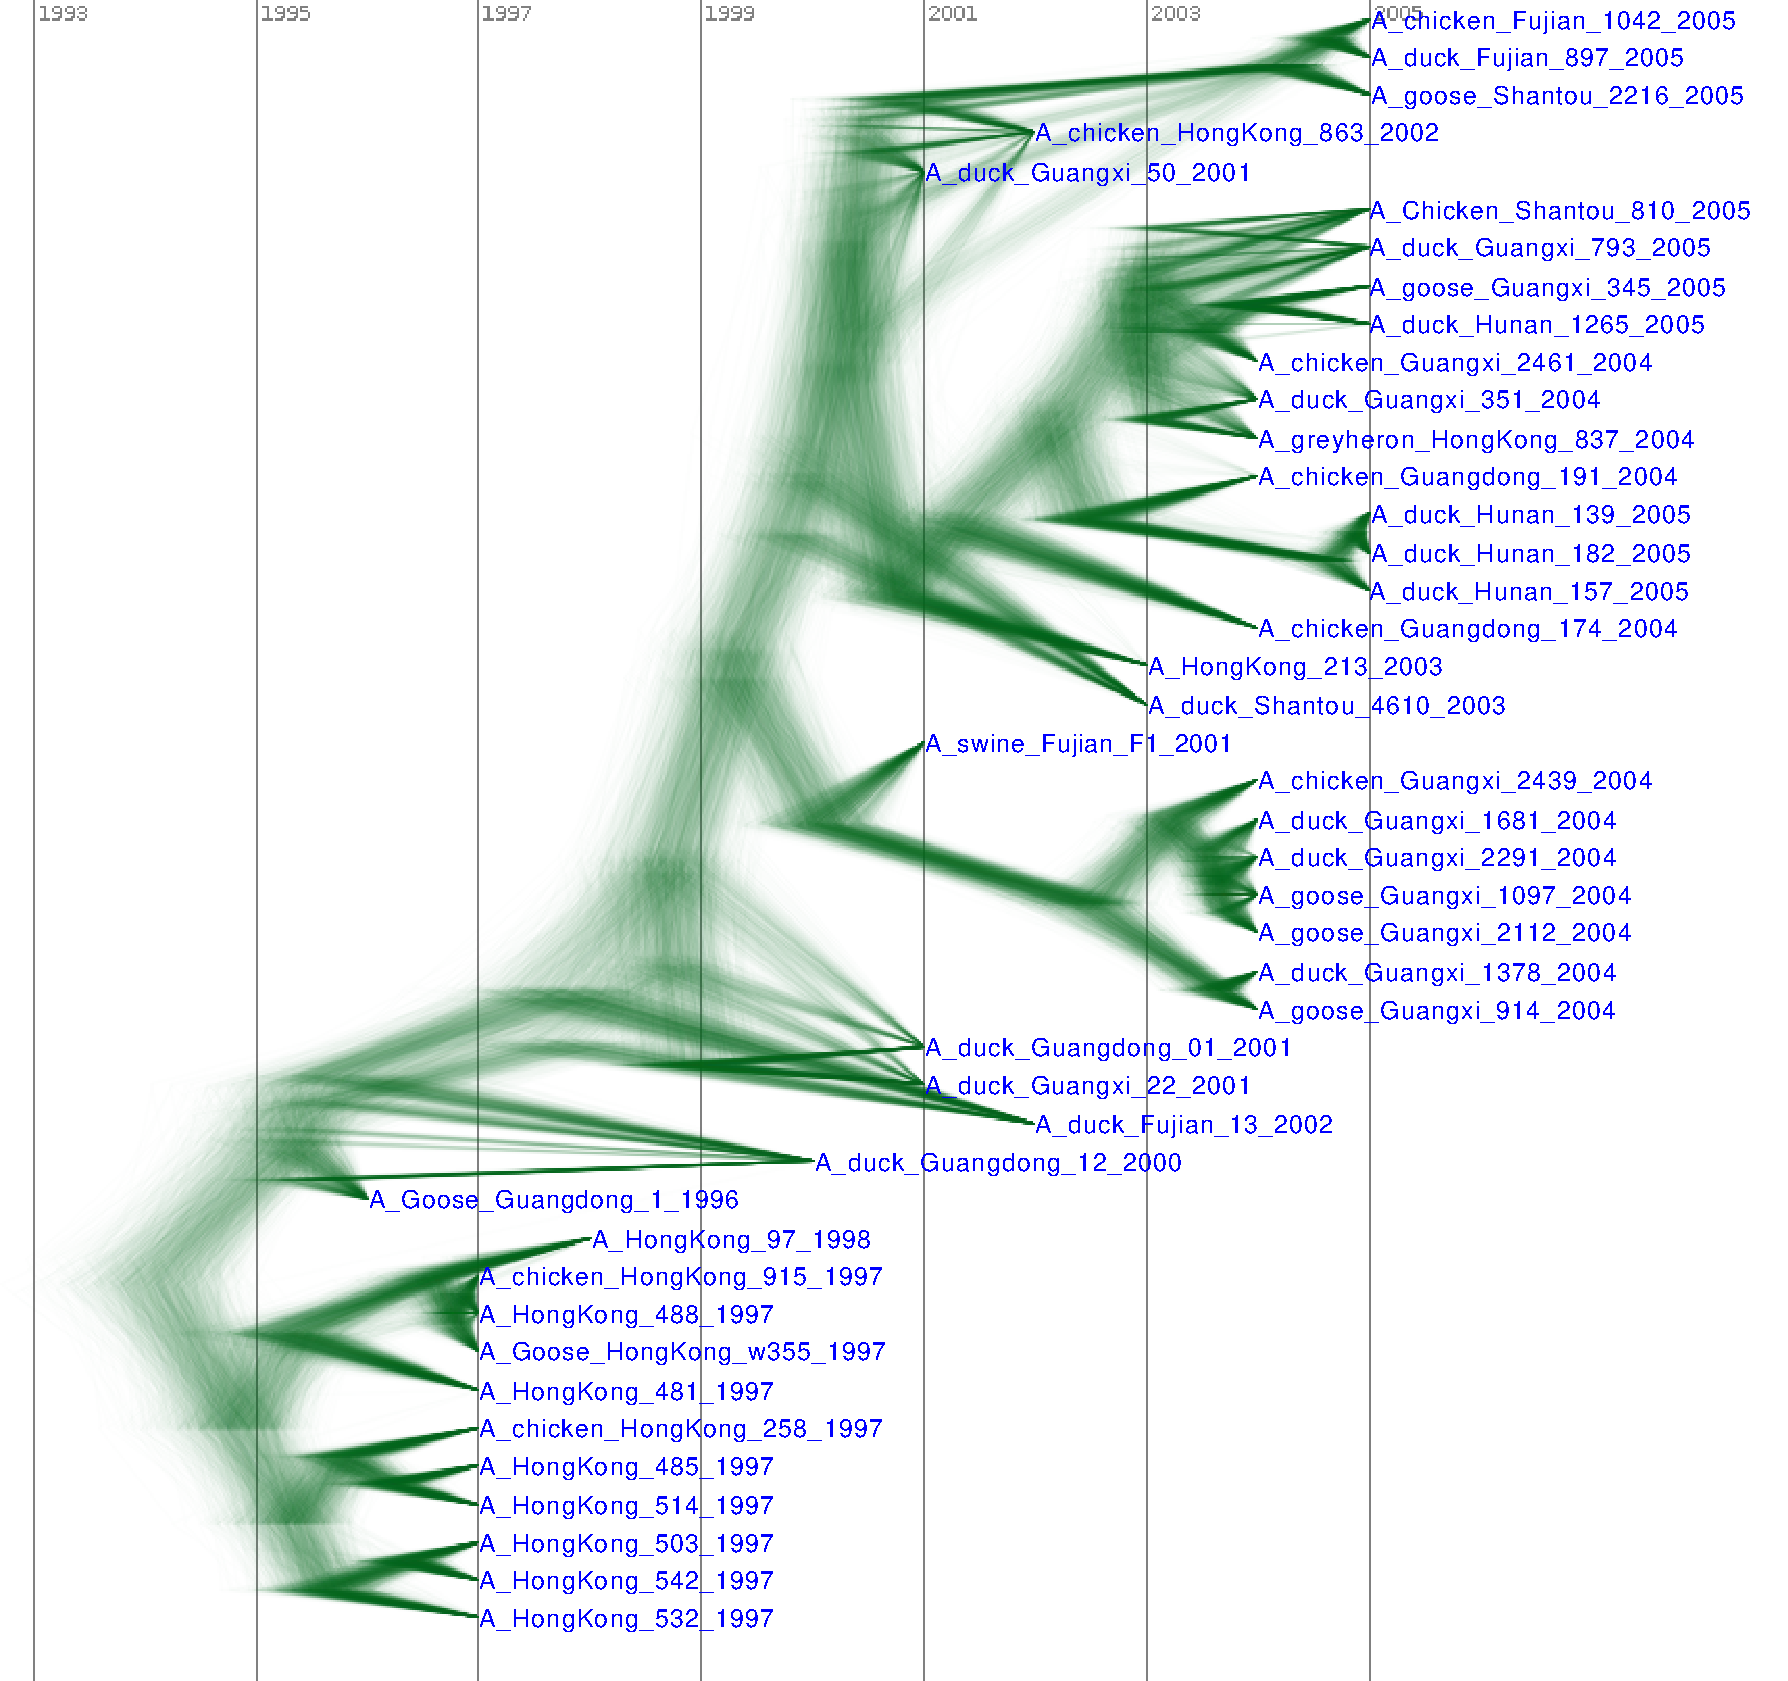
\includegraphics[scale=0.4]{figures/DensiTree.pdf}}
\end{center}
\caption{\label{fig.DensiTree} DensiTree representation of the species tree.}
\end{figure}

You can colour branches by location to get something like Figure \ref{fig.DensiTree2}.

\begin{figure}
\begin{center}
\frame{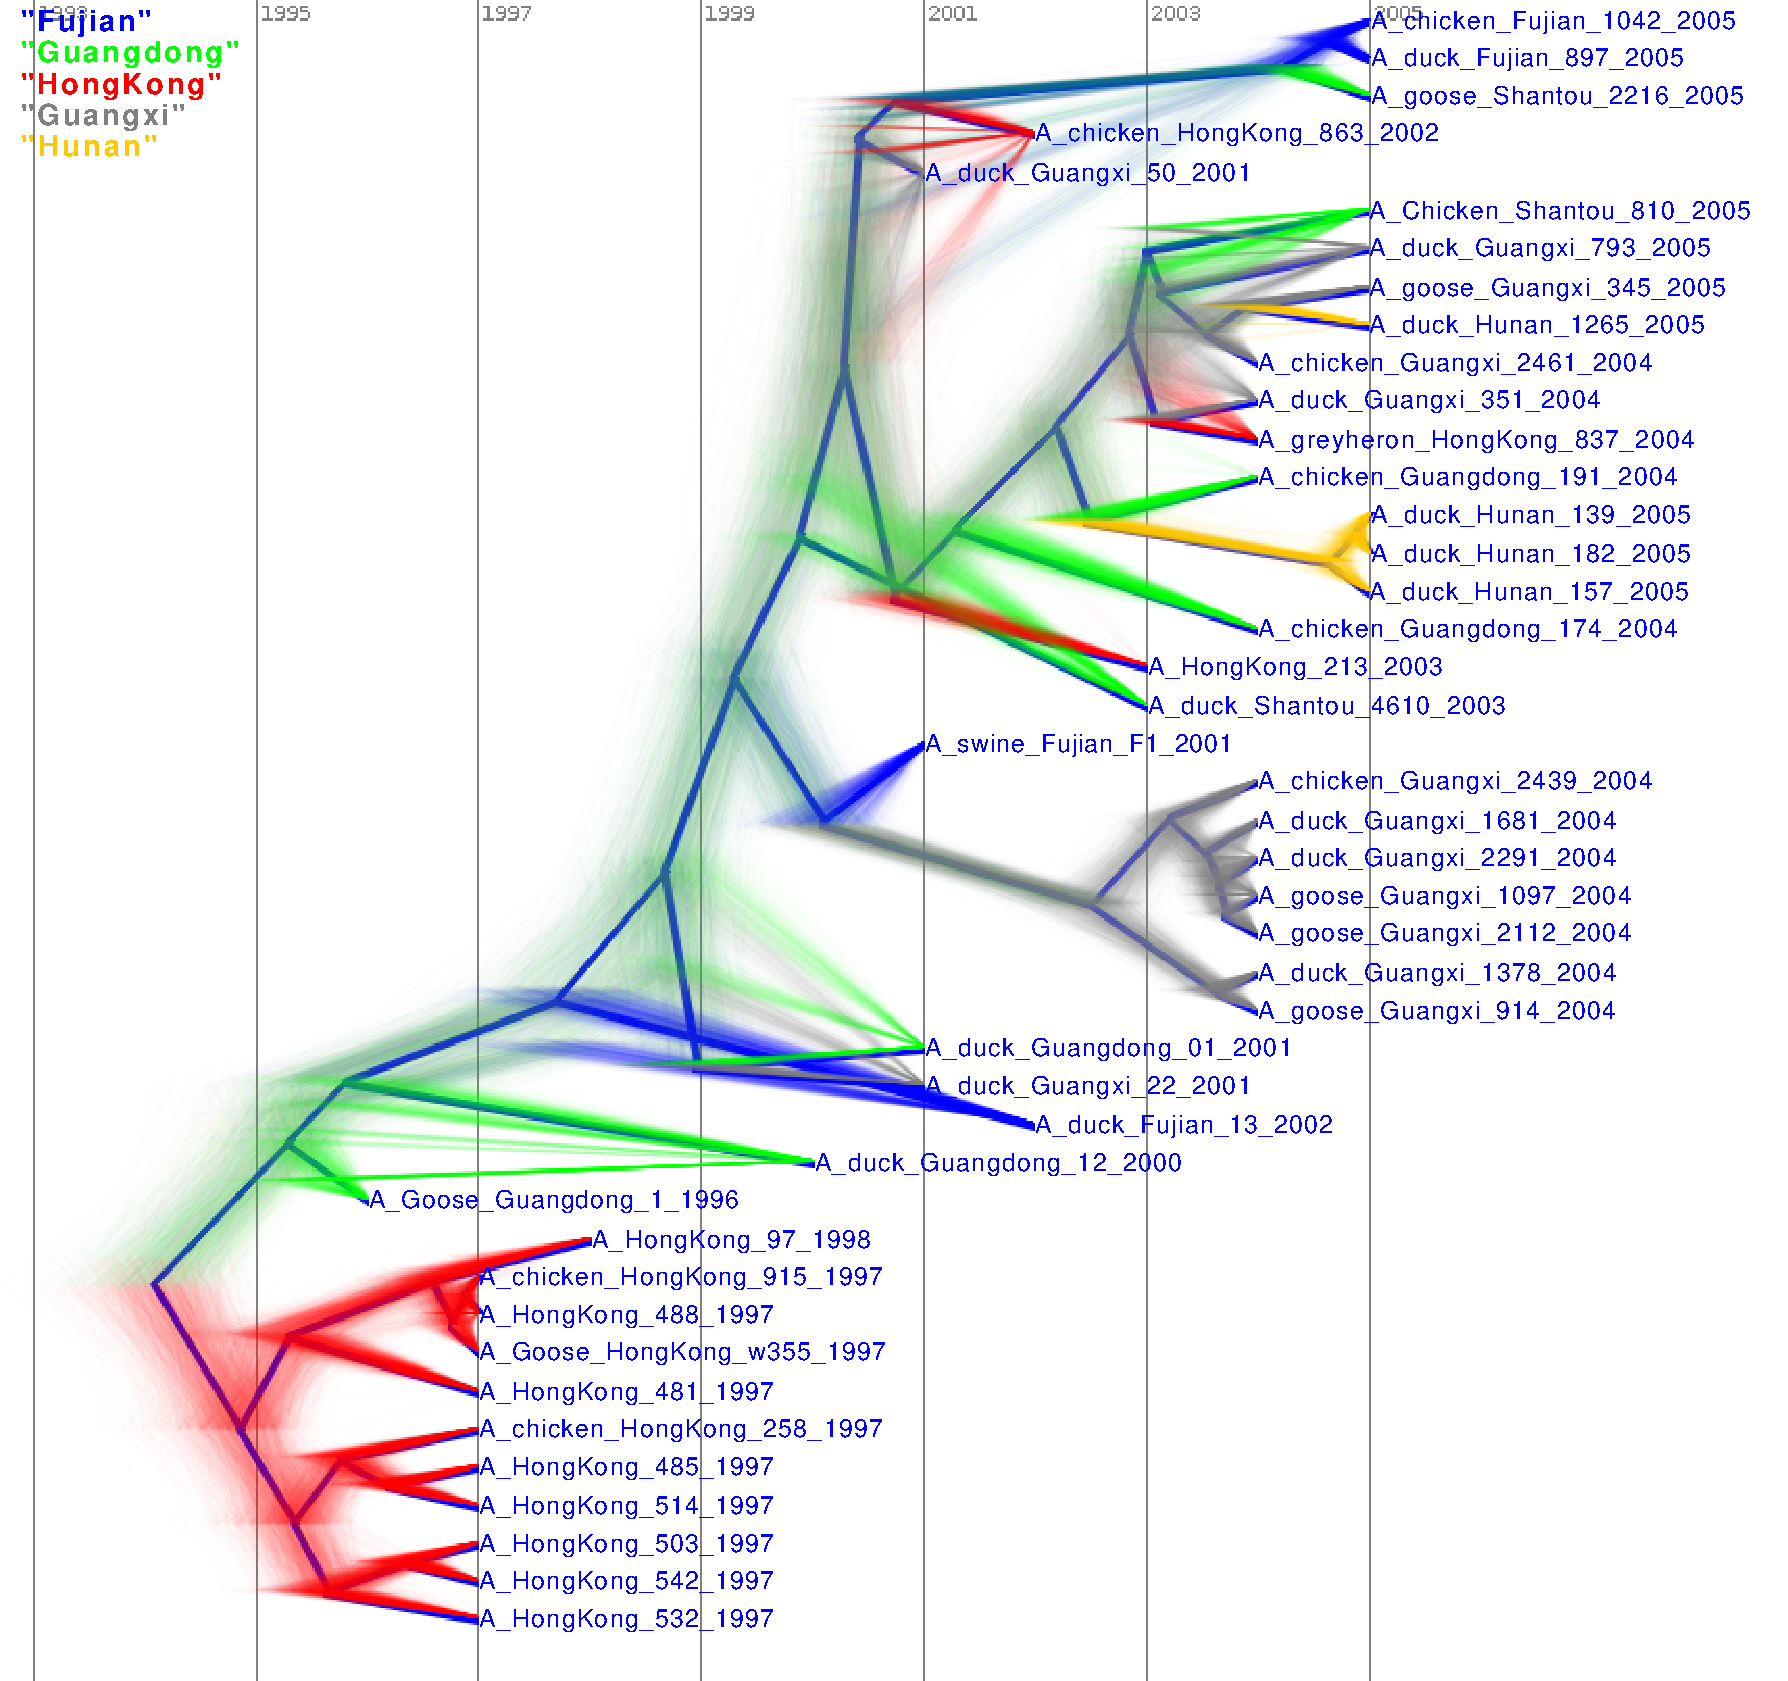
\includegraphics[scale=0.4]{figures/DensiTree2.pdf}}
\end{center}
\caption{\label{fig.DensiTree2} DensiTree with branches coloured by location.}
\end{figure}

\subsection*{Post processing geography}

Start spread by double clicking the spread.jar file.

Select the 'Open' button in the panel under 'Load tree file', and select the summary tree file.

Change the 'State attribute name' to the name of the trait. We used 'location' so change it to location.

Click the set-up button. A dialog pops up where you can edit altitude and longitude for the locations. 
Alternatively, you can load it from a tab-delimited file. A file named H5N1locations.dat is prepared already.

{\bf Tip:} to find latitude and longitude of locations, you can 
use google maps, switch on photo's and select a photo at the location 
of the map. Click the photo, then click 'Show in Panoramio' and a 
new page opens that contains the locations where the photo was taken.
An alternative is to use google-earth, and point the mouse to the 
location. Google earth shows latitude and longitude of the mouse 
location at the bottom of the screen.

Now, open the 'Output' tab in the panel on the left hand side. Here, you can choose where to save the KML file (default {\tt output.kml}).

Select the `generate' button to generate the KML file, and a world map appears with the tree superimposed onto the area where the rabies epidemic occurred.

\frame{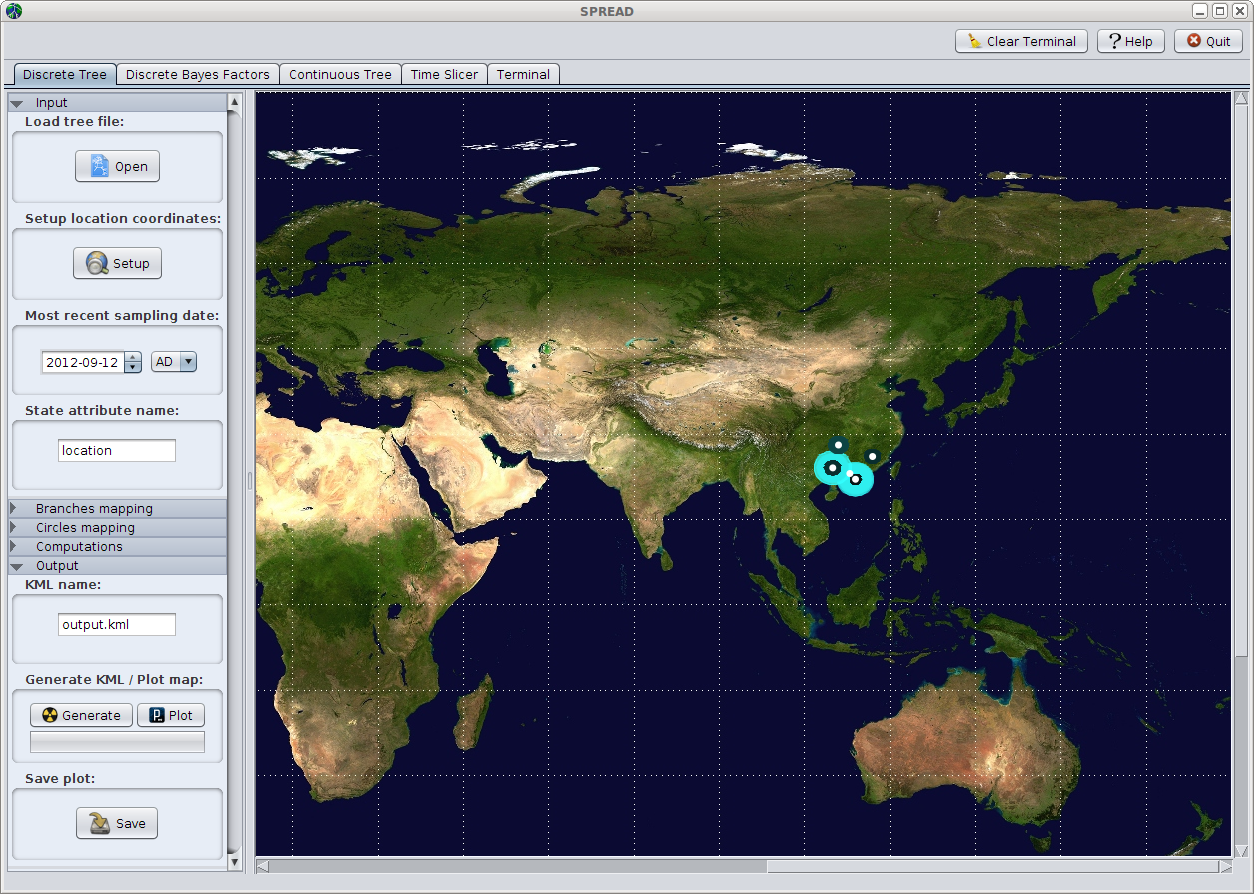
\includegraphics[scale=0.4]{figures/spread.png}}

The KML file can be read into google earth. Here, the spread of the epidemic can be animated through time. The coloured areas represent the 95\% HPD regions of the locations of the internal nodes of the summary tree.

\begin{figure}

\frame{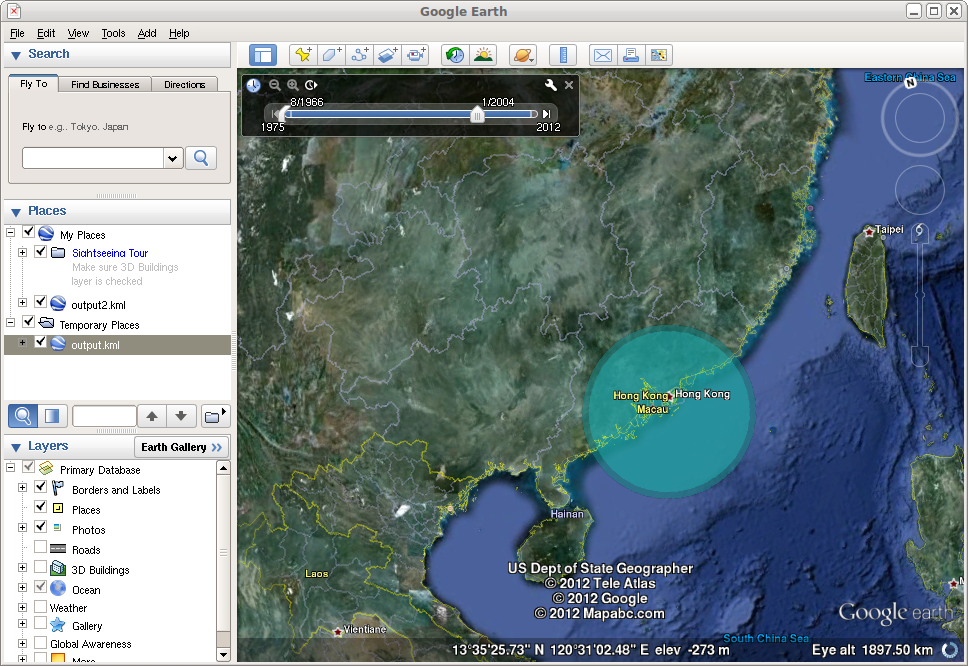
\includegraphics[scale=0.25]{figures/google-earth0.png}}
\frame{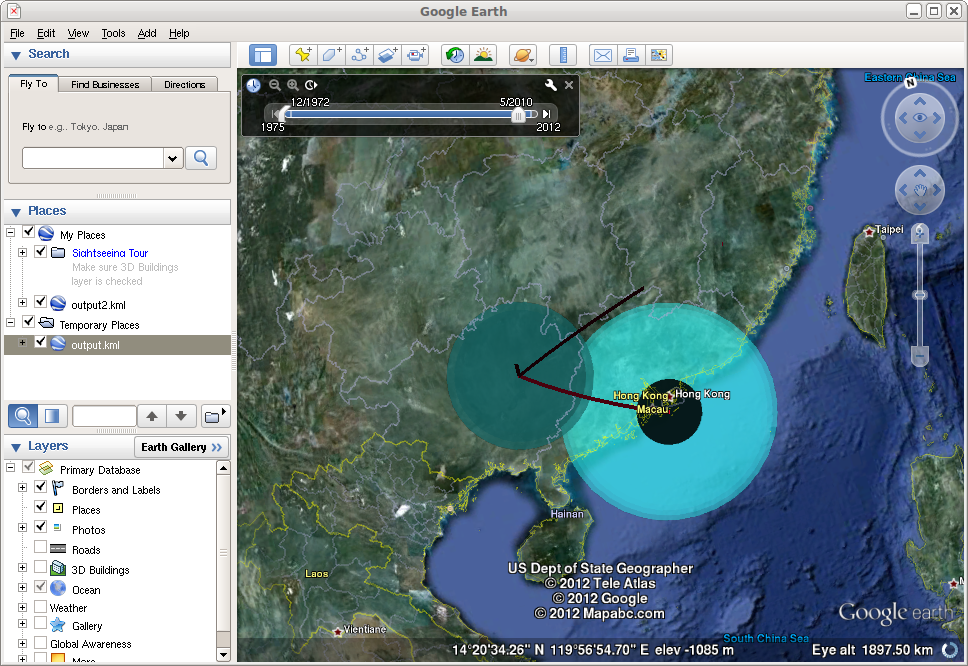
\includegraphics[scale=0.25]{figures/google-earth1.png}}
\frame{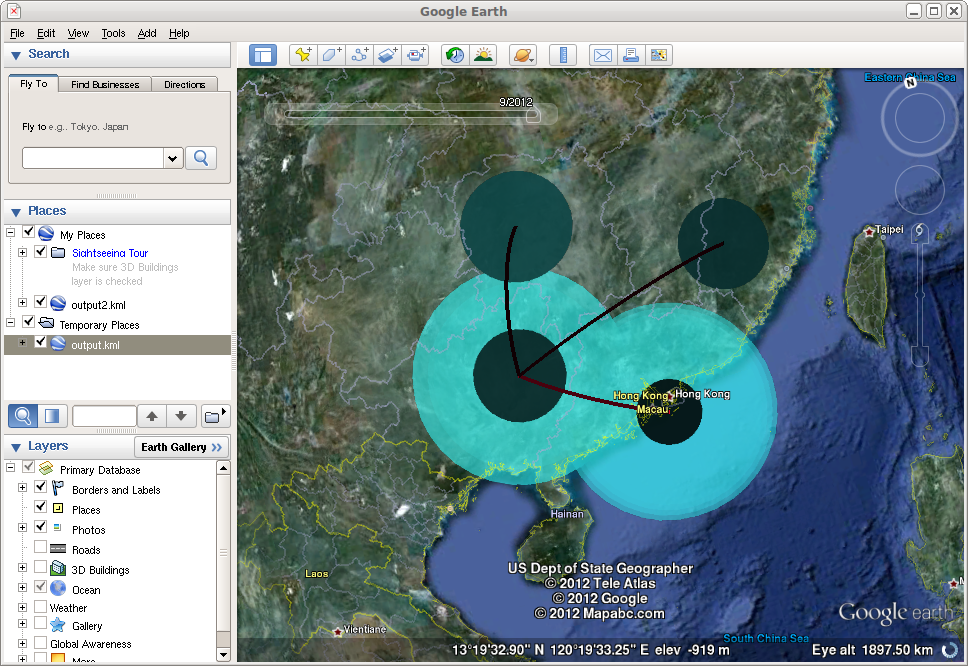
\includegraphics[scale=0.5]{figures/google-earth2.png}}
\caption{label{fig.ge}Google earth used to animate the KML file}
\end{figure}


\bibliography{AR}


\end{document}
